\section{Colour Science}

Overview text required.





\subsection{Black Calibration}

Black Calibration is a term that describes finding the sensor output value, per pixel, in the absence of any illumination.

It covers:\\

- Dark frame subtraction\\
- Dark current compensation\\
- Using black reference columns (called "optical black" by other manufacturers) to find the black level and fine-tune static offsets. \\

\textbf{Note:} Black reference columns can be used to reduce row noise as well. See Section 11.2 Pattern Noise.





\subsubsection{Calibration methods}





\paragraph{Dark Frame Subtraction}

This is a basic technique: take a picture with the lens cap on, and subtract it from your image. To make really sure no light is reaching the sensor, also cover the entire camera with something.\\ 

\textbf{How many dark frames?}\\

Problem: if you take only one dark frame, it will also contain read noise (assummed to be Gaussian and uncorrelated with the read noise from other frames). Therefore, subtracting only one image will actually increase the noise in the final output, by sqrt(2).\\

Solution: use a master dark frame, averaged from many images.\\

How many?\\

If you take N images, the signal will be multiplied by N, and the noise will be multiplied by sqrt(N). Therefore, the SNR will increase by log2(sqrt(N)) stops.\\

So, 16 dark frames will reduce the read noise in the dark frame by 2 stops, 64 frames by 3 stops, and 256 frames by 4 stops.\\

Okay, but how much noise will be added to the output image?\\

Let's say the read noise stdev in one image is r, so a dark frame averaged from N frames will have noise \consoleCommand{stdev = r/sqrt(N)}. Therefore, the noise in the output image will be: \consoleCommand{sqrt(r\^2 + r\^2/N) = r * sqrt(1 + 1/N)}.\\

Check it in octave:\\ 

\begin{lstlisting}[language=bash,morekeywords=$,keywordstyle=\bfseries,frame=none,xleftmargin=.25in,belowskip=2em, aboveskip=2em]
    octave:1>  N = 4;
    octave:2>  a = randn(1,1000000);    # one Gaussian noise sample, with mean=0 and stdev=1
    octave:3>  b = randn(N,1000000);    # N noise samples
    octave:4>  std(a + mean(b))         # add one noise sample to N averaged noise samples
    ans =  1.1174
    octave:5>  sqrt(1 + 1/4)            # compare with the theoretical result
    ans =  1.1180
\end{lstlisting}

So, it seems that averaging a small number of dark frames will not introduce significant noise in your images (4 should be enough if you are in a hurry, and 16 should give a very good result).\\

Example: one dark frame at 6ms x1 (same image as above), vs 4 darkframes at 6ms, averaged.\\

\begin{center}
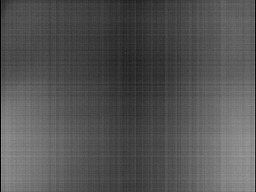
\includegraphics[height=12cm]{images/blackframes-gainx1-offset2047-5ms-01}
\end{center}

\begin{center}
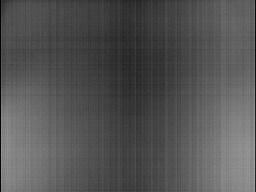
\includegraphics[height=12cm]{images/darkavg-5ms}
\end{center}

What about camera settings?\\

Unfortunately, dark frames depend on many camera settings: analog gain (ISO), exposure, other sensor settings like offset, black sun protection, PLR configuration and so on. Temperature is a variable as well.\\

Luckily, the dependence on exposure appears to be linear, so we can take calibration frames at various exposures, combine them into a single dark frame, adjust it for the dark current and use it for the entire range of exposure settings (hopefully). We'll discuss that in the next section.\\ 

\textbf{Dark current}\\

Let's look at some dark frames: gain x1, exposures 1.2ms, 6ms and 78ms. Notice they get brighter as exposure increase.\\

\begin{center}

\includegraphics[height=12cm]{images/blackframes-gainx1-offset2047-1ms-01}
\end{center}

\begin{center}
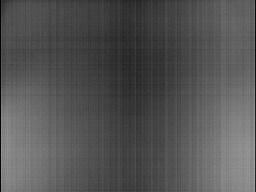
\includegraphics[height=12cm]{images/darkavg-5ms}
\end{center} 

\begin{center}
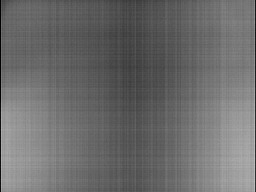
\includegraphics[height=12cm]{images/blackframes-gainx1-offset2047-64ms-01}
\end{center}

The overall brightness in the dark frame changes with exposure in a linear fashion. We'll try to account for this in two ways: with a simple scalar value, and with a per-pixel correction.\\

The values in the black reference columns do not appear to compensate for the dark current, so we'll need to do it ourselves.\\

By identifying the dark current, we will be able to compute a dark frame that is applicable to any usual exposure time, but we are going to store only one or two reference frames for each gain. First reference frame will be called a bias frame (a zero-length exposure, that would contain only static black offsets), and the second reference frame, if used, will be called a dark current frame.\\

Dark current cannot be fully corrected because, while its stationary value can be measured and subtracted, it also introduces photon noise. Roger Clark explains it better:\\ 

\textit{"Dark current is temperature dependent and most modern CMOS digital cameras, circa 2008 and later have on sensor dark current subtraction, but while the dark current level is subtracted, the noise from the dark current still accumulates."} - Source: \href{http://www.clarkvision.com/reviews/how-to-interpret-reviews/}{http://www.clarkvision.com/reviews/how-to-interpret-reviews/}

\textbf{Simple correction}\\

Experimentally, we have found the dark frame changes with exposure at roughly 0.065 digital units for each ms. This value is multiplied by analog gain. To find this value, take the dark frames at different exposure times (say 1...50 ms), then do a linear fit for the frame average (or median).\\

Command-line:

\consoleCommand{raw2dng *x1*.raw12 --calc-darkframe}

Example: a dark frame created from 256 exposures, between 1.2ms and 77ms, without using black reference columns. The image was adjusted (with a constant offset) to match a zero-length exposure, so calling it bias frame may be a good idea. If we use it to correct the individual dark frames, we should no longer see a variation in overall brightness. 

\consoleCommand{    Averaged 256 frames exposed from 1.19 to 76.79 ms.
    Dark current: 0.0653 DN/ms}
    
Image sequence: bias frame, single dark frames at exposures 1.2, 6 and 77 ms, corrected with the bias frame and the (scalar) dark current average. All files scaled to show a range of 60 DN, but the master dark frame has a different offset than the others.     


\begin{center}
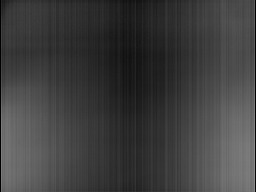
\includegraphics[height=12cm]{images/darkframe-x1-no-blackcol-256}
\end{center}

\begin{center}

\includegraphics[height=12cm]{images/blackframes-gainx1-offset2047-1ms-01-simple-darkframe-no-blackcol}
\end{center} 

\begin{center}

\includegraphics[height=12cm]{images/blackframes-gainx1-offset2047-5ms-01-simple-darkframe-no-blackcol}
\end{center}

\begin{center}

\includegraphics[height=12cm]{images/blackframes-gainx1-offset2047-64ms-01-simple-darkframe-no-blackcol}
\end{center}





\paragraph{Dark Current Non-uniformity Correction}

One common use of bias frames is for scaling dark frames. By subtracting a bias frame from a dark frame, you end up with a thermal frame. A thermal frame contains pixel values showing just the effect of dark current. Because dark current in any given pixel accumulates at a constant rate, a thermal frame allows you to predict with reasonable accuracy how much dark current there would be for different length exposures. However, given the opportunity, you’re always better off taking dark frames that match the exposure times of your light frames.\\

\href{http://qsimaging.com/ccd_noise_measure.html}{http://qsimaging.com/ccd\_noise\_measure.html}{Source}: \\

\textit{"Dark current non-uniformity is a noise that results from the fact that each pixel generates a slightly different amount of dark current. This noise can be eliminated by subtracting a dark reference frame from each image. The dark reference frame should be taken at the same temperature and with the same integration time as the image."} - Source: \href{https://www.photometrics.com/resources/learningzone/darkcurrent.php}{https://www.photometrics.com/resources/learningzone/darkcurrent.php}\\

\textit{"Dark noise is not random; in fact, it is highly repeatable. A given photosite on a sensor will accumulate almost exactly the same amount of dark noise from one exposure to the next, as long as temperature and exposure duration do not vary."}\\

So, rather than using a single scalar value (0.06 dn/ms/gain) for all pixels, we can try finding the individual dark current for each pixel. Instead of doing a linear fit on the overall dark frame brightness (vs exposure), we will do the linear fit per pixel. We'll have to acquire a lot more dark frames to compute a good result, but it might be worth the trouble.\\

Command-line:\\

\consoleCommand{raw2dng *x1*.raw12 --calc-dcnuframe}

Example: bias frame (static offset) and dark current frame (exposure-dependent offset). Notice the bias frame looks quite similar to the previous one, but a little darker. The median value of the dark current frame is, unsurprisingly, 0.0645 DN/ms. 

\begin{center}
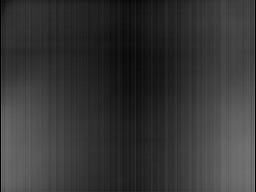
\includegraphics[height=12cm]{images/darkframe-x1-no-blackcol-darkcurrent-256}
\end{center}

\begin{center}
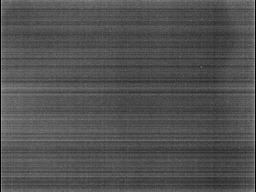
\includegraphics[height=12cm]{images/dcnuframe-x1-no-blackcol-darkcurrent-256}
\end{center}

Individual dark frames (1.2, 6 and 77 ms) adjusted with dark current nonuniformity: 

\begin{center}

\includegraphics[height=12cm]{images/blackframes-gainx1-offset2047-1ms-01-darkcurrent-no-blackcol}
\end{center}

\begin{center}
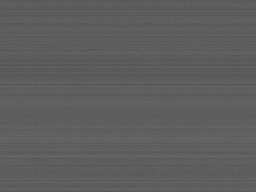
\includegraphics[height=12cm]{images/blackframes-gainx1-offset2047-5ms-01-darkcurrent-no-blackcol}
\end{center}

\begin{center}
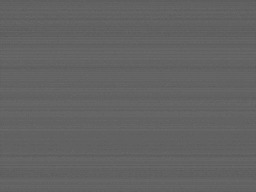
\includegraphics[height=12cm]{images/blackframes-gainx1-offset2047-64ms-01-darkcurrent-no-blackcol}
\end{center}

No obvious improvement in the test images, so why bother?\\

Let's correct all these 256 dark frames and check a few indicators: median, stdev, row noise and column noise.\\ 

Dark frame + scalar dark current: 
\begin{center}
%\includegraphics[height=5cm]{images/darkframe-check-x1-256-simple}
\end{center}


Dark frame + dark current frame:
\begin{center}
%\includegraphics[height=5cm]{images/darkframe-check-x1-256-dcnu}
\end{center}

You may notice:\\

- Median (black level) variation: noticeable improvement with the second method.\\
- stdev (overall noise): minor improvement at extreme settings.\\
- Row noise: identical with both methods.\\
- Column noise: small improvement with the second method.\\

Indeed, the more complex method appears just a tiny bit better than the simpler one.\\





\paragraph{Dark Current Measurement From Hot Pixels}

A very interesting idea can be found here - \href{https://www.photonics.com/Article.aspx?AID=44298}{https://www.photonics.com/Article.aspx?AID=44298} ... where hot pixels can be used to measure the amount of dark current and scale it properly. This will probably account for changes in temperature, and may work at very long exposures without actually having to calibrate the camera in these conditions. Genius, if you ask me. 





\paragraph{Black Reference Columns}

This sensor has 8+8 columns that can be used for calibrating the black levels; they are also useful for reducing the dynamic row noise.\\

Experimentally, we have noticed that odd rows have slightly different statistics (noise level, offset, gain), compared to even rows. This happens in both the black columns and the active area, and it may indicate two parallel circuits used for readout, each having slightly different electrical response.\\

Therefore, it may be wise to process the black columns for odd and even rows separately, which should already fix some issues like static row noise, or the need for green equilibration.\\

In raw2dng, this correction is enabled by default, as long as you use a dark frame. You can turn it off with \importantKeyword{--no-blackcol}, if you want. \\





\paragraph{Black Level}

The sensor has two registers that can be used to adjust the black level: one for odd rows, another for even rows. This confirms our finding about two parallel readout circuits.\\

You might be tempted to adjust the black level to 0 (like Nikon does). Please don't. Here's why:\\

- If you adjust the offset until the black level becomes roughly 0, you will clip all the data below this level. Good luck subtracting a dark frame after that.\\
- Even if you change the level after doing all the black corrections, you may still have useful data below zero. You will need it when stacking multiple frames, or when doing noise reduction.\\

Just FYI, there is a hack for Nikon cameras that moves the black level above 0. See \href{https://landingfield.wordpress.com/2014/05/13/teaser-nikon-dslr-black-point-hack-for-astrophotography/}{https://landingfield.wordpress.com/2014/05/13/teaser-nikon-dslr-black-point-hack-for-astrophotography/} \\

... Sample photos can be found \href{https://www.cloudynights.com/topic/473696-rho-ophiuchi-with-nikon-hacked-black-level/}{here} or \href{https://nikonhacker.com/viewtopic.php?t=2548&p=18449#p17973}{here}.

We recommend setting the offset so that only a few isolated pixels (if any) reach the value of 0. A black offset of 2047 (registers 87/88) is a good choice. You won't lose any dynamic range by doing that.\\

On most recent Canon DSLRs, black level is 2048. That's a little on the large side, but it's a good thing. Some may argue that you may lose 2 stops or more of dynamic range by doing that (reading - \href{https://www.reddit.com/r/photography/comments/3q4tnz/how_to_correctly_push_5_stops_with_canon/cwcbyb5/}{https://www.reddit.com/r/photography/comments/3q4tnz/how\_to\_correctl\_push\_5\_stops\_with\_canon/cwcbyb5/} ), but this is wrong. On Canons, the raw output is 14-bit, so by setting the offset to 2048 instead of 0, the useful range will be "just" log2(16384-2048) = 13.8 bits, instead of 14. So, yeah, you lose 0.2 bits from the ADC range.\\

With the black offset of 2047 on the CMV12K, the black level ends up at around 150, so you lose a whooping 0.05 bits from the 12-bit range.\\

\textbf{Note:} for easier processing, raw2dng shifts the raw data in order to fix the black level at 128.\\

\textbf{Note also:} Row noise correction from black columns detailed in 11.2 Pattern Noise.
 




\subsubsection{Checking Black Level}

You may wonder: after all these corrections, did we get the right black level? Can we render shadow detail correctly?\\

A possible criteria for checking: if we have two images of the same scene, taken with different exposures, we should be able to match those in postprocessing by simply dragging the exposure slider. For example, if we have one image at 5ms and another one at 20ms, we would set the exposure to +2 EV on the first image - the results should be pretty much identical, except for noise (and clipped highlights, if we weren't careful with the exposure). \\

Of course, that will work once we know the sensor Response Curves (See 11.5).\\

To check how well the images can be exposure-compensated, we could evaluate (and minimize) one of those error metrics: 

\begin{lstlisting}[language=bash,morekeywords=$,keywordstyle=\bfseries,frame=none,xleftmargin=.25in,belowskip=2em, aboveskip=2em]
    a  = dark\_image - black\_level;
    b  = bright\_image - black\_level;
    e1 = norm(a*expo\_ratio - b);
    e2 = abs(median((b ./ a)(:)) - expo\_ratio)
    e3 = mad(log2((b ./ a)(:)));
\end{lstlisting}

First metric checks the difference between the two images, where the darkest one was adjusted by scaling (gain) to match the brightest one. Second metric computes the ratio between the two images at each pixel, and checks its median value vs the expected value. Third one checks the variation of per-pixel ratios between the two images, in stops, ignoring the expected value - this metric could be useful if we suspect the exposure controls may not be accurate.\\

\begin{center}
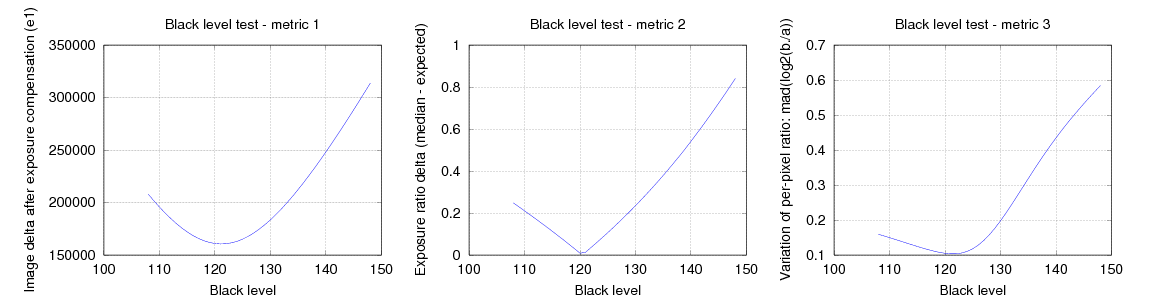
\includegraphics[height=4cm]{images/black_check}
\end{center}

With all 3 methods, minimization indicates a black level of around 120-122 (expected 128), so there's still something missing with our calibration. This is confirmed by missing details in very dark areas (crushed blacks) on some sample images.\\ 

On the same test image, the response curve estimated from the grayscale IT8 reference data indicates a black level of 129. 

On the same test image, the response curve estimated with the Robertson02 algorithm indicates a black level of 124 (See 11.5).\\

Who is right?\\

The sensor also has a strange behavior - something we have called the "Black Hole" anomaly: in very dark areas, sensor output decreases with exposure time. This might give a clue for solving this mystery.\\

\begin{center}
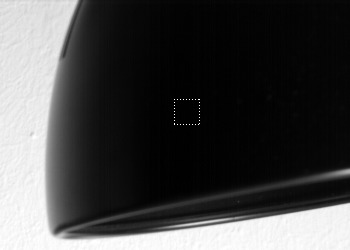
\includegraphics[height=11cm]{images/blackhole}
\end{center}





\subsubsection{Calibration Pipeline}

- Use black reference columns to find the black levels for odd and even rows.\\
- Subtract dark offset and dark current.\\
- Use variations in black reference columns to reduce row noise.\\ 

These operations should be simple enough to be implemented in FPGA, as real-time corrections. 





\subsubsection{Calibration Procedure}

\textbf{Quick calibration}\\

Acquire 16 dark frames, gain x1, exposures between 1 and 50 ms, save them under the 'darkframes' subdirectory, then run: 

\consoleCommand{raw2dng darkframes/*x1*.raw12 --calc-darkframe --swap-lines}

Result: darkframe-x1.pgm.\\

Repeat for other gains if needed.\\ 


\textbf{Accurate calibration, with dark current nonuniformity}

Acquire 256 dark frames, gain x1, exposures between 1 and 64 ms in linear increments (4 images at each setting), save them under the 'darkframes' subdirectory, then run: 

\consoleCommand{raw2dng darkframes/*x1*.raw12 --calc-dcnuframe --swap-lines}

Result: darkframe-x1.pgm and dcnuframe-x1.pgm.\\

Repeat for other gains if needed. \\

\textbf{Checking the calibration}\\

You can verify the calibration by rendering the same individual dark frames, this time corrected, to check the residuals. Or, even better, acquire a new set of dark frames at the same settings, and check those instead: 

\consoleCommand{raw2dng darkframes/*x1*.raw12 --check-darkframe --swap-lines}

You will see the average value, pixel noise and row/column noise levels (both absolute and relative to pixel noise) for each dark frame. Example:

\consoleCommand{    Average     : 127.48
    Pixel noise : 2.48
    Row noise   : 0.61 (24.6\%)
    Col noise   : 0.05 (2.2\%)}
    
Using the reference frames to correct raw12 files.\\

1. Place the calibration files in the working directory.\\
2. Make sure your \importantKeyword{.raw12} images contain a metadata block.\\
3. raw2dng will recognize the dark frames and use them for correcting your image. \\
   
\consoleCommand{    cp /path/to/darkframes/*-x[1-4].pgm .
    raw2dng *.raw12 --swap-lines}
    
\textbf{Note:} you need --swap-lines as an workaround for an old bug introduced in the Beta, but wasn't fixed yet in the FPGA.\\    
    
This is not exactly useful when dealing with multiple folders, so until we'll have a better way to organize the calibration frames, you may try an alternative workflow:\\

1. Place the calibration files in some directory (let's call it "calibration directory")\\.
2. Make sure your .raw12 images contain a metadata block.\\
3. Use paths when passing input files raw2dng (the output files will be saved in the same directory as the input file).\\

\consoleCommand{    cd /path/to/darkframes
    ls *.pgm
      darkframe-x1.pgm       dcnuframe-x1.pgm       ...
    raw2dng /path/to/images/*.raw12 --swap-lines}
     
    
\textbf{Example}

Showing half-res image crops pushed by 4 stops (ufraw-batch --wb=auto --exposure=4 --shrink=2).

- Top left: raw sensor data (adjusted black level manually).\\
- Top right: corrected with dark frame, scalar dark current, no black columns.\\
- Bottom left: corrected with dark frame, dark current frame, no black columns.\\
- Bottom right: corrected with dark frame, dark current frame, black columns enabled.\\

\textbf{Note:} in the raw data, even and odd rows have different black offsets; that's why we have wrong colors. \\

\begin{center}
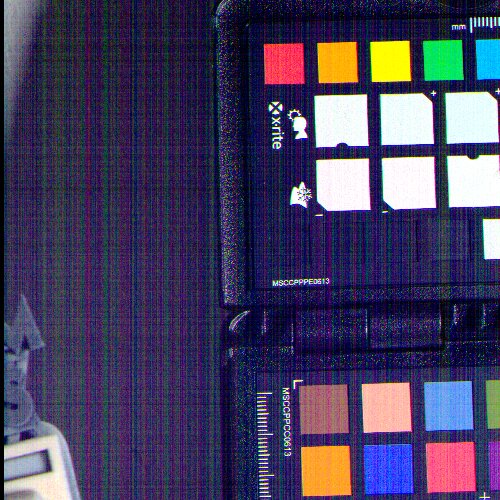
\includegraphics[height=11cm]{images/10ms+4-totally-raw-crop}
\end{center}

\begin{center}
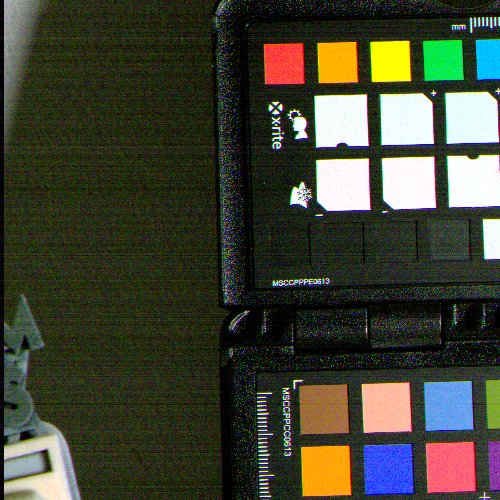
\includegraphics[height=11cm]{images/10ms+4-no-blackcol-crop}
\end{center}

\begin{center}
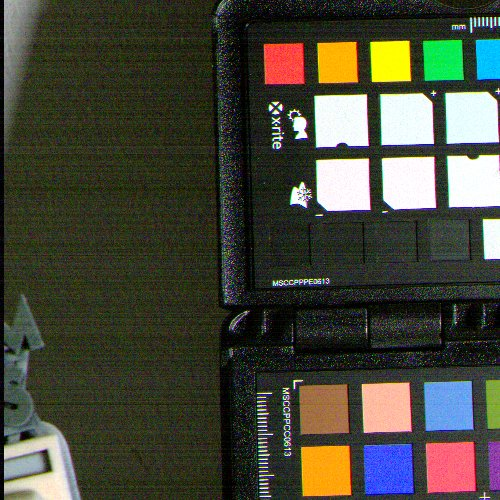
\includegraphics[height=11cm]{images/10ms+4-darkcurrent-no-blackcol-crop}
\end{center}

\begin{center}
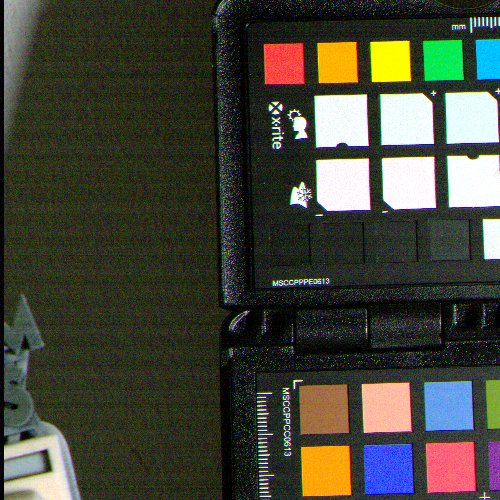
\includegraphics[height=11cm]{images/10ms+4-darkcurrent-crop}
\end{center}


    

\subsection{Pattern Noise}

General info about pattern noise can be found here - \href{http://theory.uchicago.edu/~ejm/pix/20d/tests/noise/#patternnoise}{http://theory.uchicago.edu/~ejm/pix/20d/tests/noise/\#patternnoise} \\

The CMV12000 sensor suffers from dynamic row noise.\\

That means, a scalar offset gets added to each row. The offset is not correlated between different frames, so we can't remove it using a calibration frame (dark frame or whatever).\\

One can observe this noise by looking at the difference between two images taken at identical settings. There are two main components that appear obvious in such a difference frame: random noise (per pixel, increases on brighter pixels) and row noise (per line). \\

\begin{center}
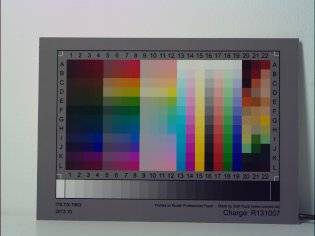
\includegraphics[height=9cm]{images/it8-gainx1-offset2047-20ms-01}
\end{center}

\begin{center}
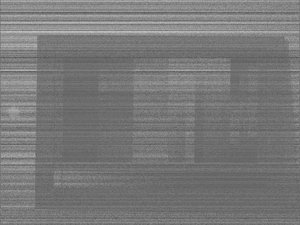
\includegraphics[height=9cm]{images/it8-gainx1-offset2047-20ms-01-minus-02-small}
\end{center}




\subsubsection{Correction Methods}

There are two ways to deal with this noise, after performing Black Calibration (See 11.1)\\

- Use info from black reference columns to reduce dynamic row noise without guessing anything (fast, can be implemented in real-time, see Raw Preprocessing).\\
- Use denoising techniques to reduce the remaining row noise (the guesswork part, slow).\\

\textbf{Reducing row noise using black reference columns}

See \href{http://github.com/apertus-open-source-cinema/misc-tools-utilities/commit/48de47b2a544dc32bbd5a8fd7701bb44a31ea850#diff-624053a553f49c0036b4d31282e58b2fR301}{http://github.com/apertus-open-source-cinema/misc-tools-utilities/commit/48de47b2a544dc32bbd5a8fd7701bb44a31ea850\#diff-624053a553f49c0036b4d31282e58b2fR301}

The application note AN01 from CMOSIS says:\\

\textit{"The noise is also present in the black reference columns (8 left and 8 right), so when enabled (reg 89[15] = 1), these can be used for row noise correction by for example making a relative row profile of these black columns and subtract this from the image."}\\

However, simply subtracting each row average of the black columns from our image is not going to work. Here's why:\\

Kalman filter theory: \href{http://robocup.mi.fu-berlin.de/buch/kalman.pdf}{http://robocup.mi.fu-berlin.de/buch/kalman.pdf} \\

From page 3, if we know how noisy our estimations are, the optimal weights are inversely proportional with the noise variances:\\

\consoleCommand{x\_optimal = (x1 * var(x2) + x2 * var(x1)) / (var(x1) + var(x2))} 

Here, let's say R = x1 is row noise (stdev = 1.6 at gain=x1) and x2 is black column noise. 

\begin{lstlisting}[language=bash,morekeywords=$,keywordstyle=\bfseries,frame=none,xleftmargin=.25in,belowskip=2em, aboveskip=2em]
    R = x1
    B = mean(black\_col') = R + x2 =>  x2 = B - R
    x2 can be estimated as mean(black\_col') - mean(active\_area')
    stdev(x2) = 1.3.
\end{lstlisting}

We want to find k that minimizes var(R - k*B). 

\begin{lstlisting}[language=bash,morekeywords=$,keywordstyle=\bfseries,frame=none,xleftmargin=.25in,belowskip=2em, aboveskip=2em]
    var(R - k*B) = var(x1 * (1-k) - x2 * k),
    => k = var(x1)) / (var(x1) + var(x2).
\end{lstlisting}

In particular, for gain = x1, k = 1.6\^2 / (1.6\^2 + 1.3\^2) = 0.6.\\

So, we don't have to simply subtract the black columns. Rather, we'll subtract the static offset (median value) first, and then, we'll subtract the remaining variations multiplied by 0.6 at gain=x1.\\

Things get a little more complex because the static offset is different on odd and even rows, and it also appears to change from the left side to right side of the frame. More details on the \textbf{Raw Preprocessing} page.\\

\textbf{Fixed frequency perturbation in black columns }\\

A closer look at the frequency spectrum of the black columns, compared to the spectrum of the row noise from a dark frame, revealed a strong fixed-frequency component present only in the black columns. Attempting to fix row noise with the above procedure would introduce some of this fixed frequency component in the main image as well.\\

In the example image from below, this component has a frequency of 1/41.27 pixels-1, with an amplitude of 1.14 DN. The value is different in other test images, and appears to be consistent in the images taken during the same experiment. It doesn't change with exposure time. Cause is unknown. \\

TODO: detailed analysis, FFT graphs...\\

We'll attempt to filter out this perturbation from the black columns before using them for reducing row noise.\\

Good news: after removing this perturbation, the optimal black columns multiplier increases to about 0.8 :) \\

\textbf{Using nearby rows to reduce the row noise even more}\\

Maybe some nearby rows could offer some hints about the row offset on the line being analyzed?\\

Looks like yes. Trying to write the row noise as a linear combination of row averages from black columns, using linear regression, not just the ones from the same row, but also from nearby rows, and discarding very small coefficients, gives the following filter:\\

 \begin{lstlisting}[language=bash,morekeywords=$,keywordstyle=\bfseries,frame=none,xleftmargin=.25in,belowskip=2em, aboveskip=2em]
    (y % 2)
       ?
         black\_col[y-1] *  0.24 +
         black\_col[y]   *  0.63
       :
         black\_col[y]   *  0.38 +
         black\_col[y+1] *  0.43
\end{lstlisting}

What's interesting: on even rows, row noise (in the active area) depends on the black column average from the same row, but also on the black column average from the previous row. But on odd rows, it depends on the black column average from the same row and the next row. This probably means they are processed in pairs, and there is some common perturbation that affects both of them.\\

This gives a minor improvement (0.6 -> 0.5). \\

\textbf{Exploiting differences in green channels}

The two green channels are expected to be nearly identical, except for high-frequency details like sharp edges. That means, if we take the median difference on each row, we expect to get zero. In practice, we get some nonzero values. We could try to see if there is any correlation between those green channel differences and our row noise.\\

Let's extract only the green channels from an image: the result will be W x H/2. Let's define green\_delta(lag) = row\_median(green - circshift(green,-lag)). That means, from each green row, subtract some nearby green row, and take the median difference. We'll compute this at lags -2, -1, 1, 2, mapped to array indices 0, 1, 2, 3.\\

Linear regression gives an ugly FIR filter that looks like this: \\

\begin{lstlisting}[language=bash,morekeywords=$,keywordstyle=\bfseries,frame=none,xleftmargin=.25in,belowskip=2em, aboveskip=2em]
    (y % 2)
       ?
         black\_col[y-2]    * 0.17 +
         black\_col[y-1]    * 0.14 +
         black\_col[y+0]    * 0.17 +
         black\_col[y+1]    * 0.16 +
         black\_col[y+2]    * 0.14 +
         green\_delta[0][y] * 0.22 +
         green\_delta[1][y] * 0.31 +
         green\_delta[2][y] * 0.38
       :
         black\_col[y-2]    * 0.12 +
         black\_col[y-1]    * 0.13 +
         black\_col[y+0]    * 0.14 +
         black\_col[y+1]    * 0.14 +
         black\_col[y+2]    * 0.12 +
         black\_col[y+3]    * 0.12 +
         green\_delta[0][y] * 0.33 +
         green\_delta[3][y] * 0.32
\end{lstlisting}

As weird as it looks, it seems to work!\\

Improvement (over the "Kalman" scaling of black columns): 0.6 -> 0.3.\\ 



\textbf{Reducing the remaining row noise by image filtering}\\

Basic algorithm:\\

1. Filter the image with an edge-aware vertical blur (bilateral filter on pixels from the same column)\\
2. Subtract the blurred image; the residuals will reveal the row noise (see example)\\
3. Mask out highlights and strong edges\\
4. Take the median value from each row of the residuals image\\
5. Subtract these values from each row of the original image \\

Source: \href{https://github.com/apertus-open-source-cinema/misc-tools-utilities/blob/master/raw2dng/patternnoise.c}{https://github.com/apertus-open-source-cinema/misc-tools-utilities/blob/master/raw2dng/patternnoise.c} \\





\subsubsection{Usage}

The methods discussed here are implemented here = \href{https://github.com/apertus-open-source-cinema/misc-tools-utilities/tree/master/raw2dng}{https://github.com/apertus-open-source-cinema/misc-tools-utilities/tree/master/raw2dng} \\

- Black reference columns are used by default, as long as you use a dark frame (since this method is fast and has no side effects)\\
- To reduce the remaining row noise, use \importantKeyword{raw2dng --fixrn}\\
- If the image also suffers from column noise, use \importantKeyword{raw2dng --fixpn} \\

Troubleshooting or checking the effectiveness of each step:

- Disable row noise reduction from black columns, but use the static offsets: \importantKeyword{--no-blackcol-rn}\\
- Disable fixed frequency correction for black columns: \importantKeyword{--no-blackcol-ff}\\
- Disable black reference columns completely: \importantKeyword{--no-blackcol} (you need to compute new darkframes if you use this)\\ 

Tip: the algorithm for filtering row noise is also available in MLVFS, so you can use it on MLV videos (recorded with Magic Lantern) as well. See - \href{http://www.magiclantern.fm/forum/index.php?topic=13152}{http://www.magiclantern.fm/forum/index.php?topic=13152}





\subsubsection{Tests on a dark frame}

Checking a single 10ms dark frame, corrected using 256 exposures between 1.2ms and 77ms, various settings. Showing only noise measurements.

\begin{lstlisting}[language=bash,morekeywords=$,keywordstyle=\bfseries,frame=none,xleftmargin=.25in,belowskip=2em, aboveskip=2em]
    # raw data without any processing
    raw2dng blackframes-gainx1-offset2047-10ms-01.raw12 --swap-lines --no-darkframe --check-darkframe
      Average     : 190.35
      Pixel noise : 7.14
      Row noise   : 5.29 (74.1%)
      Col noise   : 5.41 (75.7%)
\end{lstlisting}

\begin{lstlisting}[language=bash,morekeywords=$,keywordstyle=\bfseries,frame=none,xleftmargin=.25in,belowskip=2em, aboveskip=2em]
    # disable black columns, simple darkframe
    raw2dng *x1*.raw12 --calc-darkframe --no-blackcol --swap-lines
    raw2dng blackframes-gainx1-offset2047-10ms-01.raw12 --swap-lines --no-blackcol --check-darkframe
      Average     : 140.33
      Pixel noise : 3.08
      Row noise   : 1.33 (43.0%)
      Col noise   : 0.09 (3.0%)
\end{lstlisting}

\begin{lstlisting}[language=bash,morekeywords=$,keywordstyle=\bfseries,frame=none,xleftmargin=.25in,belowskip=2em, aboveskip=2em]
    # disable black columns, enable dark current frame
    raw2dng *x1*.raw12 --calc-dcnuframe --no-blackcol --swap-lines
    raw2dng blackframes-gainx1-offset2047-10ms-01.raw12 --swap-lines --no-blackcol --check-darkframe
      Average     : 142.46
      Pixel noise : 3.06
      Row noise   : 1.32 (43.1%)
      Col noise   : 0.08 (2.5%)
\end{lstlisting}

\begin{lstlisting}[language=bash,morekeywords=$,keywordstyle=\bfseries,frame=none,xleftmargin=.25in,belowskip=2em, aboveskip=2em]
    # dark current frame, use only static offsets from black columns
    raw2dng *x1*.raw12 --calc-dcnuframe --swap-lines
    raw2dng blackframes-gainx1-offset2047-10ms-01.raw12 --swap-lines --no-blackcol-rn --check-darkframe
      Average     : 127.46
      Pixel noise : 3.06
      Row noise   : 1.39 (45.4%)
      Col noise   : 0.10 (3.2%)
\end{lstlisting}

\begin{lstlisting}[language=bash,morekeywords=$,keywordstyle=\bfseries,frame=none,xleftmargin=.25in,belowskip=2em, aboveskip=2em]
    # dark current frame, enable black columns, don't remove the fixed frequency component from black columns
    raw2dng blackframes-gainx1-offset2047-10ms-01.raw12 --swap-lines --no-blackcol-ff --check-darkframe
      Average     : 127.46
      Pixel noise : 2.90
      Row noise   : 0.82 (28.2%)
      Col noise   : 0.10 (3.3%)
\end{lstlisting}

\begin{lstlisting}[language=bash,morekeywords=$,keywordstyle=\bfseries,frame=none,xleftmargin=.25in,belowskip=2em, aboveskip=2em]
    # dark current frame, enable black columns, remove the fixed frequency component (default setting)
    raw2dng blackframes-gainx1-offset2047-10ms-01.raw12 --swap-lines --check-darkframe
      Average     : 127.46
      Pixel noise : 2.85
      Row noise   : 0.61 (21.4%)
      Col noise   : 0.10 (3.4%)
\end{lstlisting}

\begin{lstlisting}[language=bash,morekeywords=$,keywordstyle=\bfseries,frame=none,xleftmargin=.25in,belowskip=2em, aboveskip=2em]
    # also enable --fixrn (aggressive correction)
    raw2dng blackframes-gainx1-offset2047-10ms-01.raw12 --swap-lines --fixrn --check-darkframe
      Average     : 127.42
      Pixel noise : 2.79
      Row noise   : 0.12 (4.1%)
      Col noise   : 0.10 (3.5%)
\end{lstlisting}

So, row noise was reduced from 1.33 (after dark frame correction) to 0.61 after using the black reference columns.\\

If it's still noticeable, \importantKeyword{--fixrn} should bring it to very low levels, unless you have strong horizontal lines in the image, which might trick the algorithm.\\

Some experimental row noise filters:\\

\begin{lstlisting}[language=bash,morekeywords=$,keywordstyle=\bfseries,frame=none,xleftmargin=.25in,belowskip=2em, aboveskip=2em]
    % 2-tap FIR, separate for odd/even rows
    raw2dng blackframes-gainx1-offset2047-10ms-01.raw12 --swap-lines --rnfilter=1 --check-darkframe
      Average     : 127.44
      Pixel noise : 2.84
      Row noise   : 0.51 (18.1%)
      Col noise   : 0.10 (3.4%)
\end{lstlisting}

\begin{lstlisting}[language=bash,morekeywords=$,keywordstyle=\bfseries,frame=none,xleftmargin=.25in,belowskip=2em, aboveskip=2em]
    % that ugly FIR that also looks at green channel differences
    raw2dng blackframes-gainx1-offset2047-10ms-01.raw12 --swap-lines --rnfilter=2 --check-darkframe
      Average     : 127.47
      Pixel noise : 2.81
      Row noise   : 0.31 (11.1%)
      Col noise   : 0.10 (3.4%)
\end{lstlisting}


\textbf{Example}

Showing half-res image crops pushed by 4 stops (ufraw-batch --wb=auto --exposure=4 --shrink=2).\\


- Left: raw sensor data (adjusted black level manually).\\
- Right: after dark frame and dark current subtraction, but without correction from black columns.\\
- Note: in the raw data, even and odd rows have different black offsets; that's why we have wrong colors.\\ 

\begin{center}
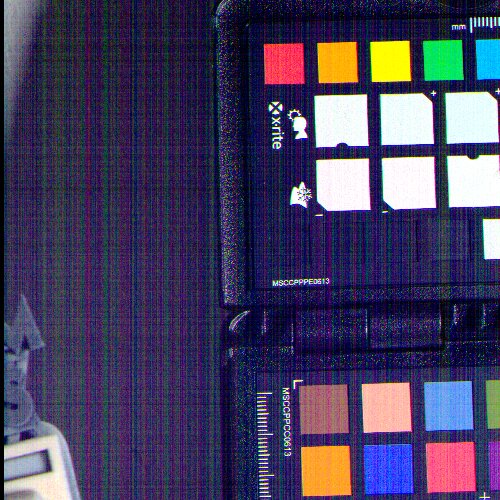
\includegraphics[height=10cm]{images/10ms+4-totally-raw-crop}
\end{center}

\begin{center}
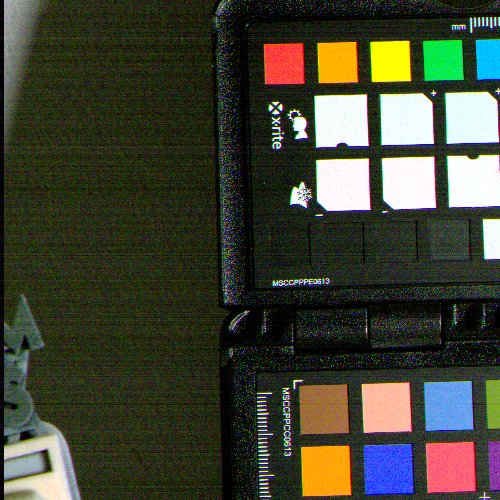
\includegraphics[height=10cm]{images/10ms+4-no-blackcol-crop}
\end{center}

- Left: after dark frame, dark current and static offsets from black reference columns.\\
- Right: after dark frame, dark current and black reference columns correction, without removing the fixed frequency component.\\

 \begin{center}
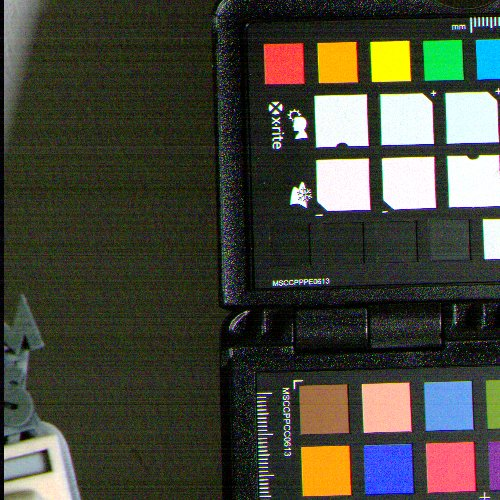
\includegraphics[height=10cm]{images/10ms+4-no-blackcol-rn-crop}
\end{center}

\begin{center}
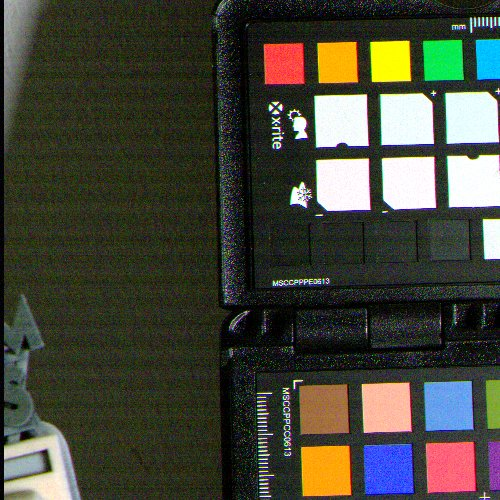
\includegraphics[height=10cm]{images/10ms+4-no-blackcol-ff-crop}
\end{center}

- Left: after dark frame, dark current and black reference columns correction.\\
- Right: after row noise reduction \importantKeyword{--fixrn} \\

\begin{center}
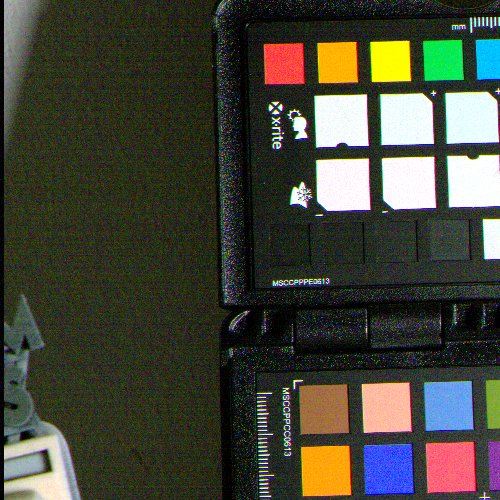
\includegraphics[height=10cm]{images/10ms+4-crop}
\end{center}

\begin{center}
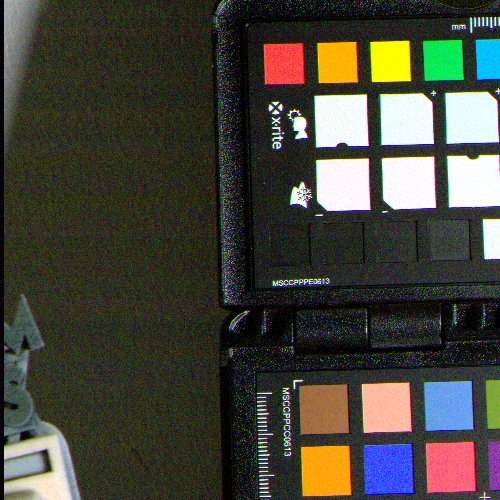
\includegraphics[height=10cm]{images/10ms+4-fixrn-crop}
\end{center}

- Left: \importantKeyword{--rnfilter=1} \\
- Right: \importantKeyword{--rnfilter=2} \\

\begin{center}
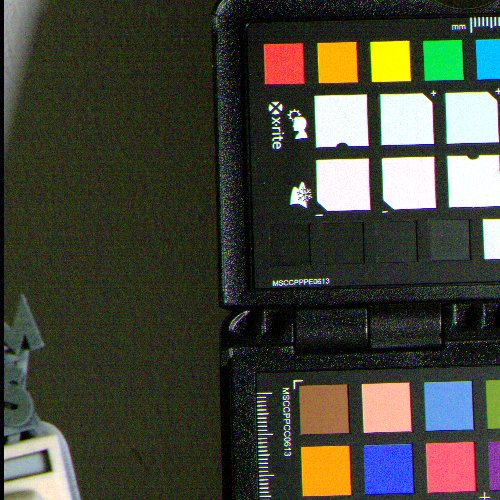
\includegraphics[height=10cm]{images/10ms+4-rnfilter1-crop}
\end{center}

\begin{center}
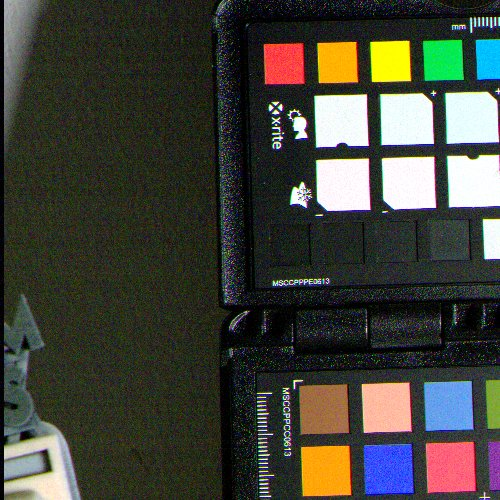
\includegraphics[height=10cm]{images/10ms+4-rnfilter2-crop}
\end{center}

Algorithm internals for \importantKeyword{--fixrn}

- Left: filtered image (vertical blur using a bilateral filter)\\
- Right: noise image, revealing row noise. Black regions are from edges that were masked.\\ 

\begin{center}
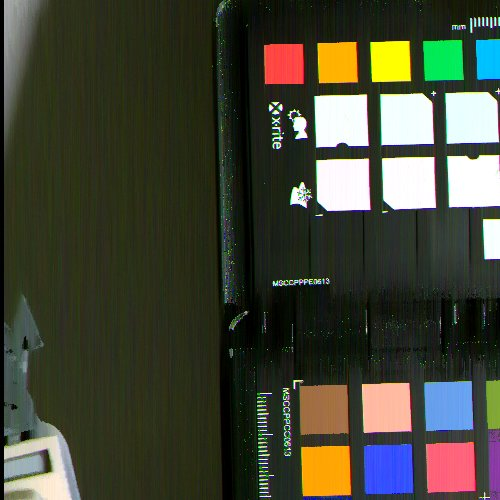
\includegraphics[height=10cm]{images/10ms+4-fixrn-dbg-denoised-crop}
\end{center}

\begin{center}
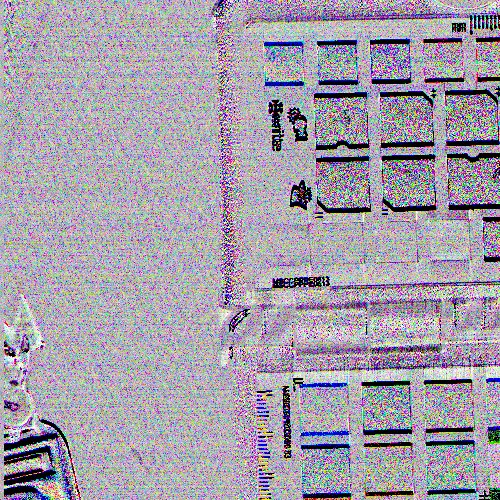
\includegraphics[height=10cm]{images/10ms+4-fixrn-dbg-noise-crop}
\end{center}

\textbf{Downsized images}\\

Corrected with dark frame and dark current only:\\
 
\begin{center}
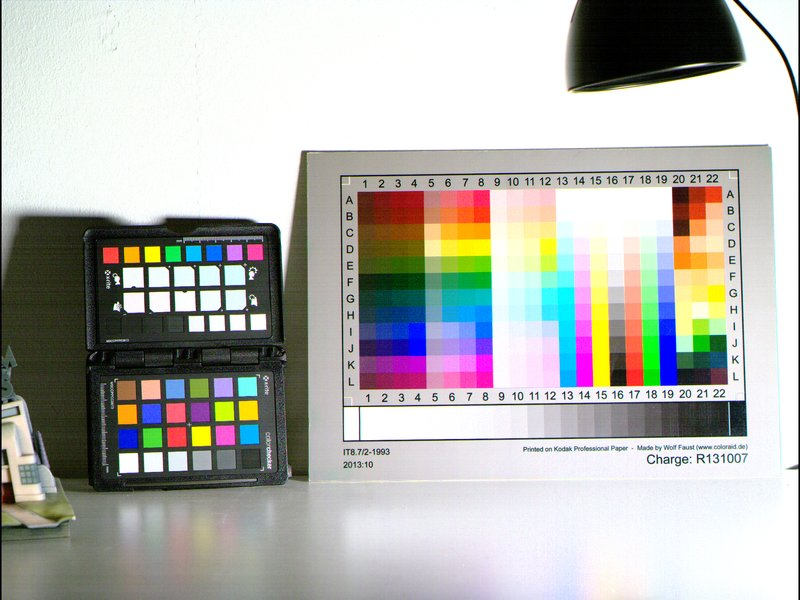
\includegraphics[height=8cm]{images/10ms+4-no-blackcol-small}
\end{center}

Also corrected with black columns: 

\begin{center}
%\includegraphics[height=8cm]{images/10ms+4-smallp}
\end{center}

Also corrected with \importantKeyword{--fixrn} 

\begin{center}
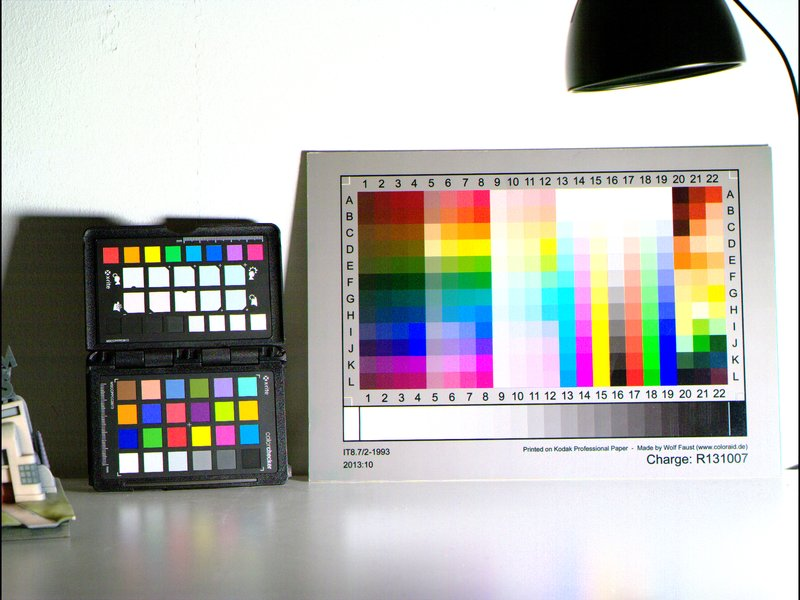
\includegraphics[height=8cm]{images/10ms+4-fixrn-small}
\end{center}

Corrected with \importantKeyword{--rnfilter=2}

\begin{center}
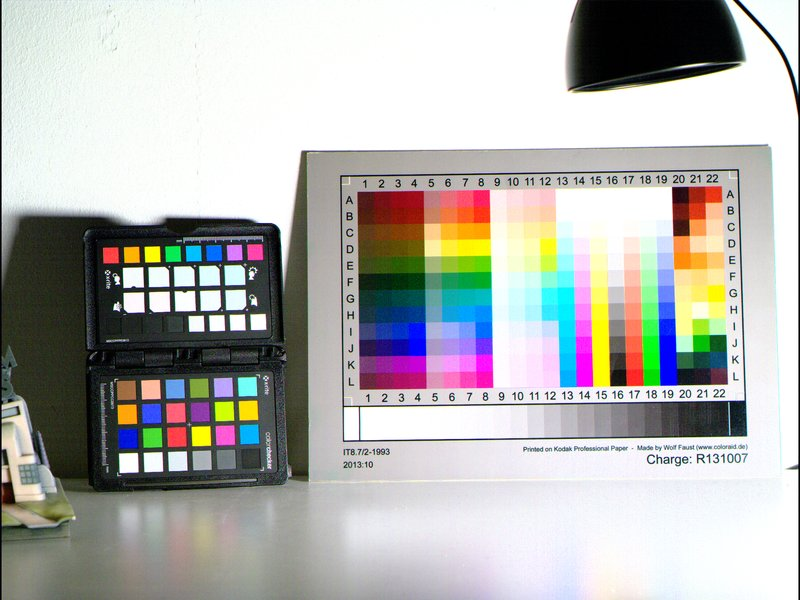
\includegraphics[height=8cm]{images/10ms+4-rnfilter2-small}
\end{center}

Larger images (half-res): \\

- 10ms+4-no-blackcol.jpg - \href{http://files.apertus.org/AXIOM-Beta/snapshots/pattern-noise/10ms+4-no-blackcol.jpg}{http://files.apertus.org/AXIOM-Beta/snapshots/pattern-noise/10ms+4-no-blackcol.jpg}\\
- 10ms+4.jpg - \href{http://files.apertus.org/AXIOM-Beta/snapshots/pattern-noise/10ms+4.jpg}{http://files.apertus.org/AXIOM-Beta/snapshots/pattern-noise/10ms+4.jpg}\\
- 10ms+4-fixrn.jpg - \href{http://files.apertus.org/AXIOM-Beta/snapshots/pattern-noise/10ms+4-fixrn.jpg}{http://files.apertus.org/AXIOM-Beta/snapshots/pattern-noise/10ms+4-fixrn.jpg}\\
- 10ms+4-rnfilter2.jpg - \href{http://files.apertus.org/AXIOM-Beta/snapshots/pattern-noise/10ms+4-rnfilter2.jpg}{http://files.apertus.org/AXIOM-Beta/snapshots/pattern-noise/10ms+4-rnfilter2.jpg} \\

\href{http://files.apertus.org/AXIOM-Beta/snapshots/pattern-noise/10ms+4-no-blackcol.jpg}{10ms+4-no-blackcol.jpg}\\
\href{http://files.apertus.org/AXIOM-Beta/snapshots/pattern-noise/10ms+4.jpg}{10ms+4.jpg}\\
\href{http://files.apertus.org/AXIOM-Beta/snapshots/pattern-noise/10ms+4-fixrn.jpg}{Final10ms+4-fixrn.jpg}\\
\href{http://files.apertus.org/AXIOM-Beta/snapshots/pattern-noise/10ms+4-rnfilter2.jpg}{10ms+4-rnfilter2.jpg}\\

All files used for this test, including scripts, calibration frames and uncompressed images, can be found here: \href{http://files.apertus.org/AXIOM-Beta/snapshots/pattern-noise/}{here}.\\

\href{http://files.apertus.org/AXIOM-Beta/snapshots/pattern-noise/10ms.raw12Raw12}{image: 10ms.raw12}\\
\href{http://files.apertus.org/AXIOM-Beta/snapshots/pattern-noise/darkframe-x1.pgm}{Calibration frames: darkframe-x1.pgm} and \href{http://files.apertus.org/AXIOM-Beta/snapshots/pattern-noise/dcnuframe-x1.pgm}{dcnuframe-x1.pgm}\\
\href{http://files.apertus.org/AXIOM-Beta/snapshots/pattern-noise/10ms.DNG}Final image (--rnfilter=2): {10ms.DNG}\\
\href{http://files.apertus.org/AXIOM-Beta/snapshots/pattern-noise/fpntest.sh}{Testing script: fpntest.sh}\\
\href{http://files.apertus.org/AXIOM-Beta/snapshots/pattern-noise/fpntest.log}{Script output: fpntest.log}\\






\subsection{Matrix Color Conversion} %See also mat4_conf.sh

Each color channel is going through 4 stages that each look like this: (I+A)*E+O 

\begin{lstlisting}[language=bash,morekeywords=$,keywordstyle=\bfseries,frame=none,xleftmargin=.25in,belowskip=2em, aboveskip=2em]
    I = input (25bit unsigned)
    A = adjustment (30bit signed)
    E = matrix coefficient (18bit signed)
    O = offset (48bit signed)
\end{lstlisting}

The four stages are connected together that the offset of stage N is the output of stage N-1. The offset of stage 1 is set in registers (32-35). The output of stage 4 is the final result.\\


For each channel that results in the following fomular: 

\consoleCommand{Ri = SUMj ((Ij + Aij) * Eij) + Oi} 

Which in other words mean the result of matrix \importantKeyword{Eij} multiplied with an input vector \importantKeyword{Ij + Aij} plus an offset vector \importantKeyword{Oi}.

Currently all registers (beside input/output) are shortened to 16bit signed (this could be changed easily) values so the matrix is currently limited to 1/256 of the possible accuracy (due to a 8bit shift of the output).\\

All input/output register are tested for over/underflow and clipped to 12 bit (this can also be disabled).\\ 

\textbf{Setting/Getting Registers: }\\

\consoleCommand{. ./hdmi.func # load functions} 

\consoleCommand{    mat\_reg 0 # Read value of register 0 = A0
    mat\_reg 0 1 # Sett value of register 0 (A0) to 1} 
    
4x4 matrix coefficients (A0, A1, A2, A3, B0, B1, B2, B3, B4, C0, C1, C2, C3, D0, D1, D2, D3) are mapped to addresses 0 - 15. In registers 16 - 31 there are adjustment values and from 32 - 35 there are 4 offset values.\\

Input format per default is (R, G1, G2, B).\\

All values of the 4x4 matrix can be set conveniently with this script:\\

\consoleCommand{./mat4\_conf.sh  A0 A1 A2 A3  B0 B1 B2 B3 B4  C0 C1 C2 C3  D0 D1 D2 D3    O1 O2 O3 O4}    
    
Where the last quadruple is optional, it defaults to 0.\\

An RGB 3x3 matrix can easily be extended to a 4x4 matrix by using the coefficient for green and offsets twice or better to half both of the green coefficients and use the same value for both greens twice. \\    
    
\begin{center}
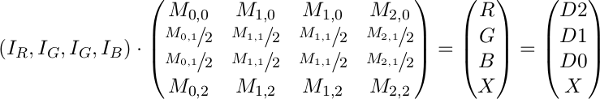
\includegraphics[height=2cm]{images/Eqn5}
\end{center}
    
    
    
    
    
   

\subsubsection{mat4\_conf.sh}

To set the 4x4 color conversion matrix, you can use the mat4\_conf.sh script:\\

The default configuration: 

\consoleCommand{./mat4\_conf.sh  1 0 0 0  0 1 0 0  0 0 1 0  0 0 0 1  0 0 0 0 } 

\textbf{Note:} In current AXIOM Beta firmware the mat4 order is changed and the default matrix is: 

\consoleCommand{./mat4\_conf.sh 0.3 0.3 0.3 0.3  0 0 0 1  0 0.42 0.42 0  1 0 0 0} 

This will be changed to reflect the documentation again soon.\\

With the Blackmagic Video Assist (BMVA), a nicer matrix (ie better skin color, less greenish): 

\consoleCommand{./mat4\_conf.sh 0.3 0.3 0.3 0.3  0 0 0 1  0 0.3 0.3 0  1 0 0 0} 

This 4x4 conversion matrix is a very powerful tool and allows to do things like mixing color channels, reassigning channels, applying effects or doing white balancing.\\

TODO: order is blue, green, red! 

\begin{center}
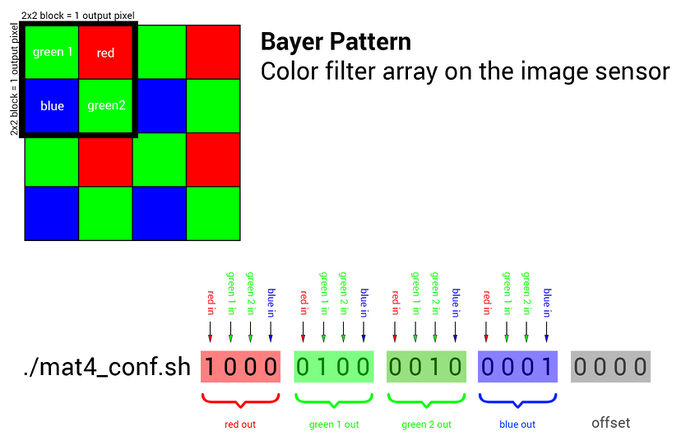
\includegraphics[height=9cm]{images/700px-Mat4-conf-illustration-01}
\end{center}

4x4 Matrix Examples:

\begin{lstlisting}[language=bash,morekeywords=$,keywordstyle=\bfseries,frame=none,xleftmargin=.25in,belowskip=2em, aboveskip=2em]
    ./mat4\_conf.sh  1 0 0 0  0 1 0 0  0 0 1 0  0 0 0 1    0 0 0 0   # unity matrix but not optimal as both green channels are processed separately
    ./mat4\_conf.sh  1 0 0 0  0 0.5 0.5 0  0 0.5 0.5 0  0 0 0 1    0 0 0 0   # the two green channels inside each 2x2 pixel block are averaged and output on both green pixels
    ./mat4\_conf.sh  0 0 0 1  0 1 0 0  0 0 1 0  1 0 0 0    0 0 0 0   # red and blue are swapped
    ./mat4\_conf.sh  1 0 0 0  0 1 0 0  0 0 1 0  0 0 0 1    0.5 0 0 0    # red 50% brigther
    ./mat4\_conf.sh  1 0 0 0  0 1 0 0  0 0 1 0  0 0 0 1.5    0 0 0 0    # blue multiplied with factor 1.5
    ./mat4\_conf.sh  .25 .25 .25 .25  .25 .25 .25 .25  .25 .25 .25 .25  .25 .25 .25 .25    0 0 0 0    # black/white
    ./mat4\_conf.sh  -1 0 0 0  0 -0.5 -0.5 0  0 -0.5 -0.5 0  0 0 0 -1    1 1 1 1    # negative
\end{lstlisting}






\subsection{CMV12000 PLR}

Some attempts to reverse engineer the PLR high dynamic range mode from CMV12000.\\ 

- 79: Number\_slopes: 1,2,3.\\
- 75-78: Exp\_kp1, Exp\_kp2: exposure times for highlights (same formula as Exp\_time)\\
- 106: Vtfl2, Vtfl3: knee point locations (range: 0-63; units: unknown) \\


\textbf{Register effects}.\\

I'll use an IT8 chart, exposed at 30 ms (normal exposure) and 100 ms (overexposed). A little dark in the lab today, but shouldn't be a big problem.\\

To analyze the images, I'll use octave 4.0, compiled with \href{http://marcelojoeng.blogspot.co.uk/2012/11/compile-octave-using-1632-bits-colour.html}{16-bit image support}. The scripts should run in Matlab as well, with minimal changes.\\

\subsubsection{Linear exposures}

\begin{center}
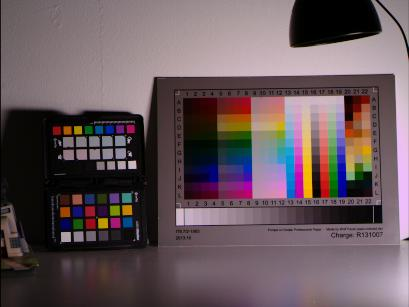
\includegraphics[height=9cm]{images/30ms-lin}
\end{center}

\begin{center}
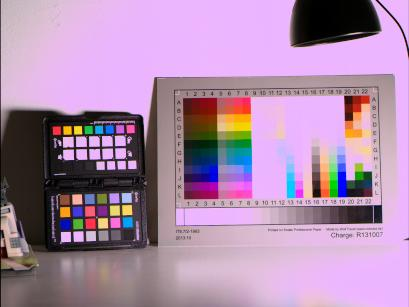
\includegraphics[height=9cm]{images/100ms-lin}
\end{center}

Let's check if the first image is really exposed to the right, in octave.  

\begin{lstlisting}[language=bash,morekeywords=$,keywordstyle=\bfseries,frame=none,xleftmargin=.25in,belowskip=2em, aboveskip=2em]
    a = read\_raw('30ms-lin.DNG');
    prctile(a(:),99) - 128        % note: black level is forced to 128 in raw2dng
    ans =  2269                   % clipping starts at about 2400-2500 above black
\end{lstlisting}

Let's check if the clipping point is, indeed, where I say: 

\begin{lstlisting}[language=bash,morekeywords=$,keywordstyle=\bfseries,frame=none,xleftmargin=.25in,belowskip=2em, aboveskip=2em]
    figure, hold on
    colors = 'rgcb';                                  % meaning: red, gren1, green2 (plotted as cyan), blue (raw data from Bayer channels)
    [g30,c30]   = sample_it8('30ms-lin.DNG', 0);      % read median RGGB swatch values from IT8 chart
    [g100,c100] = sample_it8('100ms-lin.DNG', 0);     % first output arg is grayscale, second is full color, each column is a Bayer channel
    for i = 1:4
      plot(c30(:,i), c100(:,i), ['.' colors(i)]);     % plot the 100ms image vs the 30ms one (extremely rough guess for response curve)
    end
\end{lstlisting}

\begin{center}
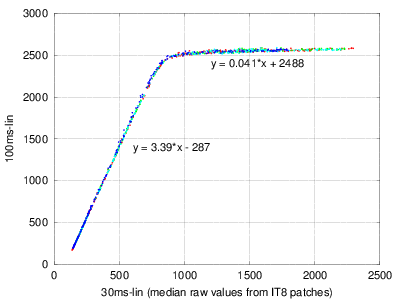
\includegraphics[height=10cm]{images/100ms-vs-30ms-lin}
\end{center}

- This approximates (but it's not equal to!) the response curve without PLR.\\
- This plot assumes the sensor response in the 30ms image (which was not overexposed) is linear (but it's probably not).\\
- The sensor doesn't clip very harshly to white (could be the PLR circuits kicking in with a very low exposure time? to be checked).\\

\subsubsection{2-segment PLR exposures}

Let's start with a 2-segment PLR exposure, 100ms/10ms, vtfl2=32. That means, Number\_slopes = 2, Exp\_time = 8072, Exp\_kp1 = 805, Vtfl=96. 

\begin{center}
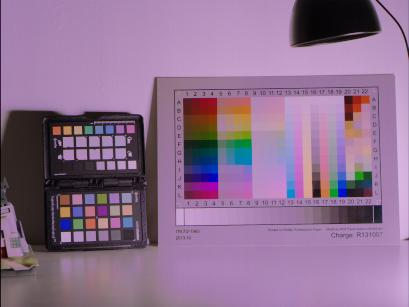
\includegraphics[height=9cm]{images/100ms-10ms-32}
\end{center}

Although the image may look a little overexposed at first sight (because of the magenta cast), the raw levels seem to be alright: 

\begin{lstlisting}[language=bash,morekeywords=$,keywordstyle=\bfseries,frame=none,xleftmargin=.25in,belowskip=2em, aboveskip=2em]
    c = read\_raw('100ms-10ms-32.DNG');
    prctile(c(:),99)
    ans =  1957
\end{lstlisting}


Let's check our response curve approximation:

 \begin{lstlisting}[language=bash,morekeywords=$,keywordstyle=\bfseries,frame=none,xleftmargin=.25in,belowskip=2em, aboveskip=2em]
    [g100p,c100p] = sample\_it8('100ms-10ms-32.DNG', 0);
    figure, hold on
    for i = 1:4
      plot(c30(:,i), c100p(:,i), ['.' colors(i)]);
    end
\end{lstlisting}

\begin{center}
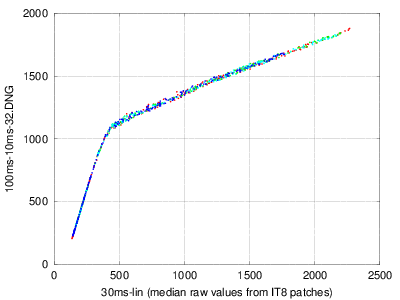
\includegraphics[height=10cm]{images/100-10-32-plr-vs-30ms-lin}
\end{center}

- The knee point isn't as sharp as in the datasheet.\\
- Its location is around 400 (todo: find the relationship between this and vtfl).\\
- The second exposure segment appears a little noisy .\\

\subsubsection{Changing Exp\_kp1}

Let's leave Vtfl constant and change exposure time for the second segment (0,1,5,10,20,35,50 ms). 

\begin{center}
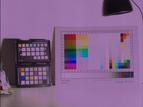
\includegraphics[height=8cm]{images/100ms-0ms-32-tiny}
\end{center}

\begin{center}
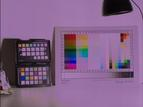
\includegraphics[height=8cm]{images/100ms-1ms-32-tiny}
\end{center}

\begin{center}
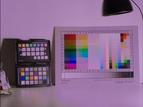
\includegraphics[height=8cm]{images/100ms-5ms-32-tiny}
\end{center}

\begin{center}
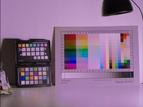
\includegraphics[height=8cm]{images/100ms-10ms-32-tiny}
\end{center}

\begin{center}
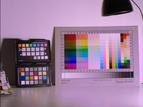
\includegraphics[height=8cm]{images/100ms-20ms-32-tiny}
\end{center}

\begin{center}
\includegraphics[height=8cm]{images/100ms-35ms-32-tiny}
\end{center}

\begin{center}
\includegraphics[height=8cm]{images/100ms-50ms-32-tiny}
\end{center}

Commands for plotting the "response curve" approximations are left as an exercise to the reader. Result: 

\begin{center}
\includegraphics[height=10cm]{images/100-x-32-plr-vs-30ms-lin}
\end{center}

\subsubsection{Changing Vtfl}

Now let's leave exposure time constant (100ms/1ms) and change Vtfl (off,0,8,16,24,32,40,48,56,63): 

\begin{center}
\includegraphics[height=9cm]{images/100ms-1ms-00-tiny}
\end{center}

\begin{center}
\includegraphics[height=9cm]{images/100ms-1ms-0-tiny}
\end{center}

\begin{center}
\includegraphics[height=9cm]{images/100ms-1ms-8-tiny}
\end{center}

\begin{center}
\includegraphics[height=9cm]{images/100ms-1ms-16-tiny}
\end{center}

\begin{center}
\includegraphics[height=5cm]{images/100ms-1ms-24-tiny}
\end{center}

\begin{center}
\includegraphics[height=9cm]{images/100ms-1ms-32-tiny}
\end{center}

\begin{center}
\includegraphics[height=9cm]{images/100ms-1ms-40-tiny}
\end{center}

\begin{center}
\includegraphics[height=9cm]{images/100ms-1ms-48-tiny}
\end{center}

\begin{center}
\includegraphics[height=9cm]{images/100ms-1ms-56-tiny}
\end{center}

\begin{center}
\includegraphics[height=9cm]{images/100ms-1ms-63-tiny}
\end{center}

\begin{center}
\includegraphics[height=10cm]{images/100-1-x-plr-vs-30ms-lin}
\end{center}

\subsubsection{Changing Exp\_time}

Now let's leave \importantKeyword{Exp\_kp1} and \importantKeyword{Vtfl} constant (0ms/32) and change base exposure time (20,50,100,150 ms):\\

\begin{center}
\includegraphics[height=10cm]{images/x-0-32-plr-vs-30ms-lin}
\end{center}

- There is a noticeable light leak in the second segment, but it doesn't seem to change with base exposure time.\\
- Most of the noise in these curves seems static (correctable with calibration frames). \\

\subsubsection{Changing Exp\_kp2 and Vtfl3}

As expected, these settings do not seem to have any noticeable effect when \importantKeyword{num\_slopes = 2}. 


\subsubsection{Mathematical models}

\textbf{First models of the response curve for 2-segment PLR exposures.}

Let's go back to the scenario with constant Vtfl and variable exposure. 

\begin{center}
\includegraphics[height=10cm]{images/100-x-32-plr-vs-30ms-lin}
\end{center}

Notice the knee point appears to move to the right with higher Exp\_kp1 values. Why would this happen?\\

If we assume the knee point threshold (Vtfl2) is only monitored while we still have time to fully expose the second segment (Exp\_kp1), we can imagine a model of the PLR exposure that looks like this:\\

\begin{lstlisting}[language=bash,morekeywords=$,keywordstyle=\bfseries,frame=none,xleftmargin=.25in,belowskip=2em, aboveskip=2em]
    function y = plr\_model_0(x, exp\_time, vtfl\_thr, exp\_kp1)
       % regular exposure time
       y = x .* ex\p_time;
       
       % time needed to reach the Vtfl threshold (lower input levels => longer times)
       t\_reach\_vtfl = vtfl\_thr ./ x;
       
       % which pixels reach vtfl?
       % assume this threshold is only monitored while we still have time
       % to fully perform the exp\_kp1 (that is, before exp_time - exp\_kp1)
       reached\_vtfl = t\_reach\_vtfl < exp\_time - exp\_kp1;
       
       % how the exposure behaves in the highlights
       y\_highlight = vtfl\_thr + x .* exp\_kp1;
       
       % copy highlight values only for those pixels that reached Vtfl
       y(reached\_vtfl) = y\_highlight(reached\_vtfl);
    end
\end{lstlisting}

Let's see how it compares to our real data. \\

\begin{center}
\includegraphics[height=10cm]{images/100-x-32-plr-vs-30ms-lin-model0}
\end{center}

Notice the slopes of the second segment seem to be higher in the real data, compared to our model, as if the real exposure time would be a little higher.

Since the slope at \importantKeyword{exp\_kp1=0} doesn't depend on total exposure time, let's assume there is some sort of exposure leak - that is, the actual exposure time is \importantKeyword{exp\_kp1} + some constant (called \importantKeyword{exp\_leak} ). 


\begin{lstlisting}[language=bash,morekeywords=$,keywordstyle=\bfseries,frame=none,xleftmargin=.25in,belowskip=2em, aboveskip=2em]
    function y = plr\_model\_1(x, exp\_time, vtfl\_thr, exp\_kp1, exp\_leak)
      
       [ ... ]  
      
       % how the exposure behaves in the highlights
       y\_highlight = vtfl\_thr + x .* (exp\_kp1 + exp\_leak);
      
       [ ... ]  
      
    end
\end{lstlisting}

\begin{center}
\includegraphics[height=10cm]{images/100-x-32-plr-vs-30ms-lin-model1}
\end{center}

Tuning parameters (trial and error): \importantKeyword{vtfl\_thr = 850}, \importantKeyword{exp\_leak = 2.5ms}.\\

Black level 128 (after subtracting black reference columns, dark frame and dark current nonuniformity). Reference frames obtained from fitting 256 dark frames taken at exposures from 1 to 64 ms, in 1 ms increments, 4 images at each exposure, with raw2dng --swap-lines --calc-dcnuframe *x1*.raw12.\\

This model appears to explain the actual response curves pretty well, but there's still room for improvement. \\

\textit{At this point, I would try to find some real response curves and reduce the noise of the test images by averaging multiple frames, then repeat the experiment. This will take a while.}\\

After averaging 50 frames at each setting, the noise in the curve remained the same, so it must be systematic error (correctable with some sort of calibration frame).\\

Finding response curves from bracketed images is difficult - we can't just scale exposure times hoping we'll get the same curve. We will need a dimmable light source with no ambient light (or some dedicated calibration hardware).\\


To be continued. 








\subsection{CMV12000 Response Curves}

\textbf{Identifying response curves on the CMV12000 sensor }\\

We would like the data coming from the sensor to be linear (that is, proportional to the number of photons received). Plus some constant offset.\\

Is it already linear, or do we have to adjust it?\\

This sensor has a high dynamic range mode called PLR (piecewise linear response). In this mode, the sensor response is highly nonlinear (configurable, but the output is not exactly piecewise linear, so we still have to identify the curves). Details about this mode on the PLR page.\\

Here we'll focus on identifying the response curves.\\

eg: input range where the linear sensor response, and use that range to correct nonlinearities that occur outside this range (for example, with underexposure, overexposure, or by comparing a PLR mode with a regular exposure mode). This can be good enough for initial tests, but it has a major problem. \\

Suppose we have a sensor with this response: \importantKeyword{y = (t*x)\^2 }(where t is exposure time, x is radiance, x*t is the number of photons captured, and y is the sensor output value, all in arbitrary units). Let's expose two synthetic images from it, in octave: 

\begin{lstlisting}[language=bash,morekeywords=$,keywordstyle=\bfseries,frame=none,xleftmargin=.25in,belowskip=2em, aboveskip=2em]
    x = linspace(0, 1, 1000);             % synthetic "image" with range from 0 to 1 (black to white)
    a = x.^2;                             % "expose" the image for 1 time unit
    b = (3*x).^2;                         % "expose" the image for 3 time units
    subplot(131), plot(x, a, x, b)        % plot the sensor responses vs input signal (radiance)
    subplot(132), plot(a, b);             % plot the second image, under the assumption that first one might be linear
    subplot(133), plot(log2(a), log2(b)); % also try a logarithmic plot
    hold on, plot(log2(a),log2(3*a),'k'); % expected response for the logarithmic plot
\end{lstlisting}

\begin{center}
\includegraphics[height=5cm]{images/naive}
\end{center}

Our simulated sensor has obviously nonlinear sensor response, yet comparing two images suggest its output might be actually linear.\\

However, the log plot indicates there may be a problem, so this type of nonlinearity is not really 100% hidden. One could also think the exposure controls on the sensor were not accurate (in this case, you would also get an offset between the two curves, so it's easy to mistake these two situations).\\

This nonlinearity was pretty obvious, but subtler variations may be much more difficult to spot, so we should really find a way to recover the true response curve. Without a photon counter, that is. \\

\textbf{Test data}\\

Bracketed image of the grayscale line from an IT8 chart, 1...100ms in 1ms increments, exposure sequence executed 100 times, images at identical settings averaged. 

\begin{center}
%\includegraphics[height=5cm]{images/it8-grayscale}
\end{center}

\textbf{Existing algorithms}\\

- Review: Best algorithms for HDR image generation. A study of performance bounds. \href{https://hal.archives-ouvertes.fr/file/index/docid/733853/filename/best_hdr_algo_hal.pdf}{Ref.}\\
- Debevec97 \href{http://www.pauldebevec.com/Research/HDR/debevec-siggraph97.pdf}{Ref 01.} k\href{http://pages.cs.wisc.edu/~csverma/CS766_09/HDRI/hdr.html}{Ref 02}, implemented in mkhdr \href{http://duikerresearch.com/mkhdr-archive/}{Ref 03}.\\
- Robertson02 \href{http://pages.cs.wisc.edu/~lizhang/courses/cs766-2008f/projects/hdr/Robertson2003ETA.pdf}{Ref 01}, implemented in pfshdrcalibrate \href{http://resources.mpi-inf.mpg.de/hdr/calibration/pfs.html}{Ref 02}.\\
- ArgyllCMS, shaper+matrix algorithm\\
- other algorithms that we can try? \\


\subsubsection{Debevec97 results}

\textbf{Robertson02 results}

\begin{center}
\includegraphics[height=7cm]{images/response-curve-pfs}
\end{center}

These curves seem to indicate that our black level may be a little too high. Figure out why. \\

Scripts, logs: \href{http://files.apertus.org/AXIOM-Beta/snapshots/response-curves/pfs/}{http://files.apertus.org/AXIOM-Beta/snapshots/response-curves/pfs/}\\

\paragraph{ArgyllCMS shaper+matrix results}

WIP, source code - \href{https://github.com/apertus-open-source-cinema/misc-tools-utilities/commit/155be5e8cac9c7d158b8cf1a3055c833c9eab9a9}{https://github.com/apertus-open-source-cinema/misc-tools-utilities/commit/155be5e8cac9c7d158b8cf1a3055c833c9eab9a9}.\\

Q: can this be used on bracketed images?\\


\subsubsection{Custom algorithms}

\paragraph{Median vs exposure}\mbox{}\\

This assumes the exposure setting from the sensor is accurate, so the input signal that will be digitzed is proportional to number of photons (scene radiance multiplied by exposure time.\\

Unfortunately, this method delivered inconsistent results (two experiments resulted in two different curves -

\begin{center}
\includegraphics[height=8cm]{images/curve-new}
\end{center}

\begin{center}
\includegraphics[height=8cm]{images/curve-old}
\end{center}


\subsubsection{Black Hole anomaly}

Here's an example showing how much the exposure setting can be trusted. Crop taken from a bracketed exposure (1,2,5,10,20,30 ms) repeated 700 times and averaged. Image from the figure is from the 30ms exposure.\\ 

\begin{center}
\includegraphics[height=10cm]{images/blackhole}
\end{center}

That's right - when exposure time increases, very dark pixels become even darker.\\

Also note the black level, after correcting the image with dark frames and black reference columns, is set to 128 (the entire image is adjusted by adding a constant, so the black reference columns reach this value). The pixels showing this anomaly are below this black level. There is detail in the image, even in a single (non-averaged) exposure, but for some unknown reason, it ends up below the black level.\\

This behavior cannot be reproduced on dark frames though, so probably (unconfirmed hypothesis) the black level goes down (not sure if globally or locally) when the image content gets brighter. The detail in the dark area on the test image looks normal (not reversed), so probably the total number of photons captured is the variable we should account for? \\


\subsubsection{Matching per-pixel curves}

This algorithm is roughly inspired from Robertson02, but without any solid mathematical background; only with the hope that it will converge to a good solution.\\

1. Initial guess:\\

- Plot per-pixel response curves on a graph, trusting exposure control on the sensor for accuracy.\\
- For each sensor output value, let's say from 16 to 2048 in 0.25-stop increments, compute the median exposure required to get that output.\\
- Shift each curve horizontally, in log space, to match the median exposure.\\
- Repeat until convergence.\\
 
1. Refinement:\\

- Assume each pixel curve may be shifted by a constant offset vertically.\\
- Repeat the same algorithm used for initial guess, but also shift the curves vertically, in linear space, by a constant offset.\\
- Assume the average shift value is 0 (the algorithm may converge to a wrong solution without this constraint).\\

Problems:\\

- You can't operate on too many pixel curves at once (it can get slow and memory-intensive).\\
- There's no proof on whether it will converge, and if yes, how accurate the solution will be (but we can try it on synthetic data).\\ 

Example (only a single line from the test images was used): \\

Initial guess:\\

\begin{center}
\includegraphics[height=7cm]{images/response-curve-test-init}
\end{center}

Second guess:\\

\begin{center}
\includegraphics[height=7cm]{images/response-curve-test}
\end{center}

\textbf{Note:} The response looks a bit different from Robertson02. Who is right?\\




\subsubsection{Direct per-pixel curves}

Storing response curves for each pixel would be really expensive in terms of storage (memory), but may be worth trying.\\

Test data: bracketed exposures at 1,2,5,10,20,30 ms. 700-frame average for each exposure (total 4200 images, captured overnight). This would reduce dynamic noise by log2(sqrt(700)) = 4.7 stops, so the static variations should be reasonably clean.\\

Since the test image was not perfectly uniform (since we didn't actually shoot a flat field frame), we probably won't be able to find out the PRNU. \\



\subsubsection{WIP}

\paragraph{Curves from grayscale IT8 reference data}\mbox{}\\

Response curves can be also estimated from the IT8 reference data, which was (hopefully) measured with much better accuracy than what we can achieve with our current setup.\\

Advantage:\\

- We have some absolute reference data.\\
- We can get a quick estimation of some part of the curve from a single image.\\ 

Problems:\\

- In our setup, the illumination is nonuniform.\\
- Tthe dynamic range of the IT8 chart is not very high (7.33 stops on the bottom gray scale).\\
- Few data points (because, without a matrix, we can only use grayscale swatches; on the good side, these few data points are not very noisy).\\ 

Solutions/workarounds:\\

- We can account for the nonuniform illumination by checking the brightness levels at the edges of the chart (light gray); it's not very exact, just better than nothing.\\
- To cover the entire dynamic range, we can use bracketed images, but this is not perfect - the image levels appear to vary with number of photons, see the \textbf{Black Hole anomaly}.\\
- We may be able to use the curve matching algorithm to account for these unwanted variations with exposure time.\\

 
\paragraph{Correcting for nonuniform illumination}\mbox{}\\

Sampling data from the edge of the chart (left) lets us correct for nonuniform illumination: one can either adjust the chart itself (right), or the reference data (preferred).\\

\begin{center}
\includegraphics[height=9cm]{images/it8_lum_sampling_areas}
\end{center}

\begin{center}
\includegraphics[height=9cm]{images/it8_lum_correction}
\end{center}

See also:\\

\begin{center}
\includegraphics[height=10cm]{images/it8_lum_correction_3d}
\end{center}

\begin{center}
\includegraphics[height=10cm]{images/it8_lum_correction_2d}
\end{center}

Why it's better to adjust the reference data instead of chart pixels?\\

- Black level in our setup is uncertain.\\
- The chart borders are fairly bright, so the measurements of border brightness are not really influenced by small black level variations.\\
- Adjusting the image must be done in log space, so we must operate on linearized data.\\
- If the black level is uncertain, the adjusted dark swatches will have large errors.\\
- If the response curve is not linear (and not known), adjusting the data under the assumption of linearity will introduce extra errors.\\
- On the other hand, reference IT8 data is already in linear XYZ space, so adjusting it will not introduce extra errors (other than our less-than-accurate measurements).\\
- The measurement errors can be hopefully solved with an iterative procedure (anyone able to prove it?).\\ 

Plotting raw data vs reference values on IT8 gray swatches gives:\\

\begin{center}
\includegraphics[height=7cm]{images/it8_lum_check}
\end{center}

In the left figure, the two grayscale lines from the IT8 chart diverge because of nonuniform illumination. After adjusting the reference data, the match is much better, though it's still not perfect (because we can't really measure the nonuniform illumination in the chart, other than by including it in the model when performing the color profiling step).\\

\paragraph{Iterative procedure for estimating the response curve in the presence of nonuniform illumination}\mbox{}\\

- Initial estimation of response curve, from noisy data (because of nonuniform illumination).\\
- Adjust the reference data from brightness on chart borders (use griddata to interpolate).\\
- Estimate the response curve again, this time from much cleaner data.\\
- Repeat steps 2-3 until convergence.\\ 

Unfortunately, this is not going to solve the mismatch between the two scales. Better get some properly illuminated charts :) 

